% !TeX spellcheck = de_CH_frami
\section{MOS Operationsverstärker (Kap. 12)}
\begin{minipage}[c]{0.5\textwidth}
	\textbf{OTA:} Hohe Eingangsimpedanz, hohe Ausgangsimpedanz. Verhalten einer spannungsgesteuerten Stromquelle.
\end{minipage}
\begin{minipage}[c]{0.5\textwidth}
	\textbf{OpAmp:} Hohe Eingangsimpedanz, tiefe Ausgangsimpedanz. Verhalten einer spannungsgesteuerten Spannungsquelle.
\end{minipage}

\subsection{Struktur}
\begin{minipage}[c]{0.3\textwidth}
	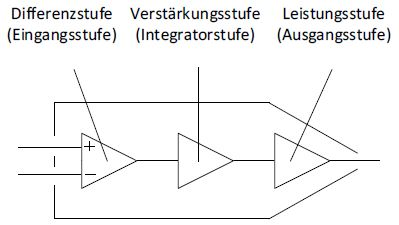
\includegraphics[width=1\linewidth]{chapters/OpAmp/images/Blockstruktur}
\end{minipage}
\begin{minipage}[c]{0.7\textwidth}
	\textbf{Differenzstufe} bildet die Differenz der beiden Eingangssignale und verstärkt sie mit dem Differenzverstärkungsfaktor.\\
	\textbf{Verstärkungsstufe} erhöht die Gesamtverstärkung. Bestimmt meist die Gesamtbandbreite des Operationsverstärkers.\\
	\textbf{Leistungsstufe} wandelt die Impedanz. Verstärkung ist selten grösser als eins. Verkleinert den Ausgangswiderstand und stellt genügend Ausgangsstrom zur Verfügung.\\[1ex]
	\textbf{Hinweis:} In seltenen Fällen sind erste und zweite oder auch zweite und dritte Stufe differenziell gekoppelt.
\end{minipage}

\subsection{Differenzstufe}
Eigenschaften der Differenzstufe bei starker Inversion:\\
\begin{tabular}{ll}
	$V_d = \pm \frac{1}{2}\sqrt{\frac{I_Q}{\beta}}$& Linearität der Diff-Stufe gut. An der Linearitätsgrenzen fliesst $I_D = \SI{0.74}{I_Q}$ bzw. $I_D = \SI{0.26}{I_Q}$.\\
	$V_d = \pm\sqrt{\frac{I_Q}{\beta}}$& In einem der Zweige fliesst $I_D = \SI{0.93}{I_Q}$, im anderen $I_D = \SI{0.07}{I_Q}$.\\
	$V_d = \pm\sqrt{2}\sqrt{\frac{I_Q}{\beta}}$& Der gesamte $I_Q$ fliesst in einem der beiden Zweigen.
\end{tabular}

\subsection{Slew-Rate}
\begin{compactenum}
	\item SR jeder einzelnen Verstärkerstufe untersuchen
	\item SR auf den Ausgang beziehen ($\cdot a$)
	\item Verstärkerstufe mit kleinster SR ist dominant.
\end{compactenum}
	\begin{tabular}{ll}
		Definition Slew-Rate&$SR=\frac{dv_o}{dt}=\frac{I_{out}}{C_L}$ [\SI{}{\volt/\micro\second}]\\
		Differenzstufe (einstufig)& $SR_r = |SR_f|=\frac{I_Q}{C_L}$\\
		Mit Verstärkung nach SR-dominanter Stufe&$|SR|=\frac{dv_{CL}}{dt}\cdot a= \frac{I_Q}{C_L}\cdot a$
	\end{tabular}\\[1ex]
	Designregel für grosse SR: $I_Q$ gross, $C_L$ klein.

\subsection{Wichtige Kenndaten/Formeln}
\begin{tabular}{p{0.3\textwidth}p{0.6\textwidth}}
	Transkonduktanz Differenzstufe & Ohne Stromspiegel $g_{md}=\frac{\delta I_{out}}{\delta V_d}=\frac{i_{out}}{v_d}=-\frac{g_m}{2}$ \\
	& Mit Stromspiegel $g_{md}=\frac{\delta I_{out}}{\delta V_d}=\frac{i_{out}}{v_d}=-g_m$ \\
	Verstärker Differenzstufe&Bei Widerstandslast $i_{out}=-\frac{g_mv_d}{2}$; $a\approx \frac{g_mr_{out}}{2}$\\
	&Bei Stromspiegellast $i_{out}=-g_mv_d$; $a\approx g_m\cdot r_{out}$\\
	Grenzwert bei starker Inversion& $a=V_A \sqrt{\frac{\beta}{I_Q}}$ (Bedingung: ${a_E}_N = {a_E}_P$)\\
	Grenzwert bei schwacher Inversion& $a=\frac{V_A}{2n_M \Phi_t}$\\
	Gain-Bandwith-Product& $GBP=|a|\cdot f_{P1}=-\frac{g_m}{2\pi C_L}$\\
	Input Common Mode Range&$V_{inp,max}=(V_{DD}-V_{SS})-V_{GS,P1}-V_{DSsat,N1}+V_{GS,N1}$\\
	&$V_{inp,min}=V_{SS}+V_{DSsat,N5}+V_{GS,N1}$\\[2ex]
	&Wenn $V_{DSsat}\approx \sqrt{\frac{2I_D}{\beta}}$ dann gilt:\\
	&$V_{inp,max}=(V_{DD}-V_{SS})-V_{T,P1}-\sqrt{\frac{I_{SS}}{\beta P_1}}+V_{T,N1}$\\
	&$V_{inp,min}=V_{SS}+\sqrt{\frac{2I_{SS}}{\beta N_5}}+V_{T,N}+\sqrt{\frac{I_{SS}}{\beta N_1}}$\\
	Common mode rejection ratio&$v_{DM}=v_{in1}-v_{in2}$ differential mode\\
	&$v_{CM}=\frac{v_{in1}+v_{in2}}{2}$ common mode\\
	$a_{DM}=\left.\frac{v_O}{V_{DM}}\right|_{v_{CM}=0}$ (ideal $a_{DM}=\infty$) Gegentaktverstärkung\\
	&$a_{CM}=\left.\frac{v_O}{V_{CM}}\right|_{v_{DM}=0}$ (ideal $a_{CM}=0$) Gleichtaktverstärkung\\
	&$CMRR=|\frac{a_{DM}}{a_{CM}}|=\frac{r_q}{r_s}=\frac{g_m}{g_{0b}}$ mit $r_q$: Innenwiderstand von $I_q$, Gleichtaktunterdrückung\\
	Power supply rejection ratio& $a_{ps}=\left.\frac{\delta V_O}{\delta V_{DD}}\right|_{V_I=konst}
	=\left.\frac{v_O}{v_{DD}}\right|_{v_I=0}$ \\
	&$PSRR_+=|\frac{a_{DM}}{a_{PS+}}|$\\
	&$PSRR_-=|\frac{a_{DM}}{a_{PS-}}|$\\
	Offset-Designregeln& \textbf{Random Offset}\\
	&Matching von Parametern der Transistoren: Layout für gutes Matching $\rightarrow$ Common Centroid, höheres $V_{GS}-V_T$ für Stromspiegel, grosses W/L für Eingangstransistoren\\
	&\textbf{Systematic Offset}\\
	&Symmetrie der Differenzstufe, gleiche $V_{DS}$ und $L$ der zu einem Stromspiegel gehörenden Transistoren, gleiche Stromdichten $\frac{I_D}{W/L}$ in Stromspiegeltransistoren\\
	& \textbf{}
\end{tabular}